 \section{Introduction aux Cloud:}
 	 \subsection{introduction}
 	  Le  Cloud Computing  que l'on pourrait traduire en français par  informatique dans les nuages doit son nom à la représentation faite d’internet dans les diagrammes réseaux. L’internet est souvent représenté par un nuage, comme le démontre la Figure \ref{fig:x diagramme}, signifiant généralement   tout le reste   ou tout ce qui est en dehors du périmètre du réseau local. Le cloud computing représente donc des ressources informatiques quelque part en dehors du réseau propre à l'entreprise ou à un particulier.
 	

  	\begin{figure}[h]
 	\centering
 	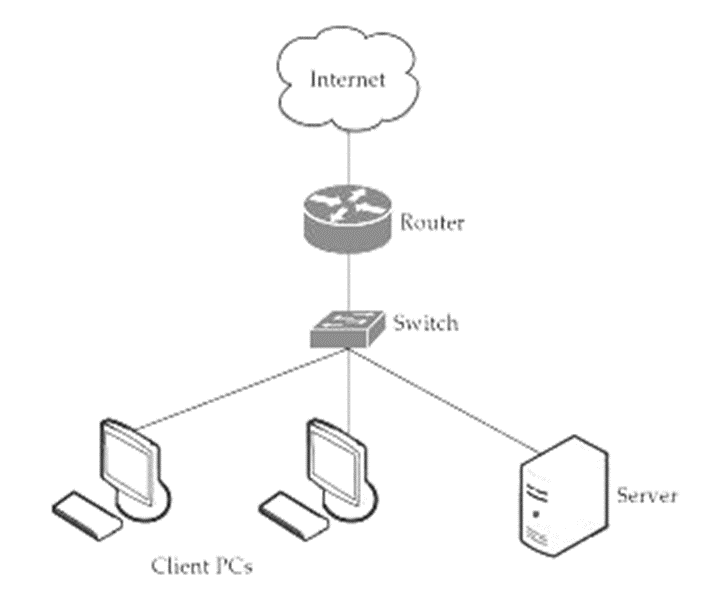
\includegraphics[scale=1]{screenshot001}
 	\caption{Représentation d'internet dans un diagramme}
 	\label{fig:x diagramme}
 \end{figure}
 	 \subsection{Définition}
 	Selon la définition du\textbf{ National Institute of Standards and Technology} (NIST), le cloud computing est l'accès via un réseau de télécommunications, à la demande et en libre-service, à des ressources informatiques partagées configurables (réseaux, serveurs, stockage, applications et services), qui peuvent être provisionnées rapidement et libérées avec un effort de gestion minimale. Ce modèle de nuage est composé de cinq caractéristiques essentielles: 
 	\begin{itemize}
 		\item 	service à la demande
 		\item Large accès au réseau
 			\item	Mise en commun des ressources
 		\item	Élasticité rapide
 			\item	Service mesuré 		
 	\end{itemize}
\textbf{ Trois modèles de services:}
  \begin{itemize}
 \item	Software as a Service (SaaS)
 \item	Platform as a Service (PaaS)
 \item	Infrastructure as a Service (IaaS)
  \end{itemize}
\textbf{ Quatre modèles de déploiementm}
 	 \begin{itemize}
 	 	\item Le cloud public
 	 	\item	Le cloud privé
 	 \item	Le cloud hybride
 	 	\item	Le cloud communautaire 
 	 	
 	 \end{itemize}
  
 
  	Pour CISCO le Cloud Computing est une plateforme de mutualisation informatique fournissant aux entreprises des services à la demande avec l’illusion d’une infinité de ressources. 
  	
  	Alors, le Cloud Computing est un concept qui consiste à transférer des fichiers ou des bases de données sur des serveurs à distance, qui étaient auparavant stockés dans la machine du client. Il permet d’accéder sur demande aux mêmes informations par plusieurs personnes.
  	\begin{figure}
  		\centering
  		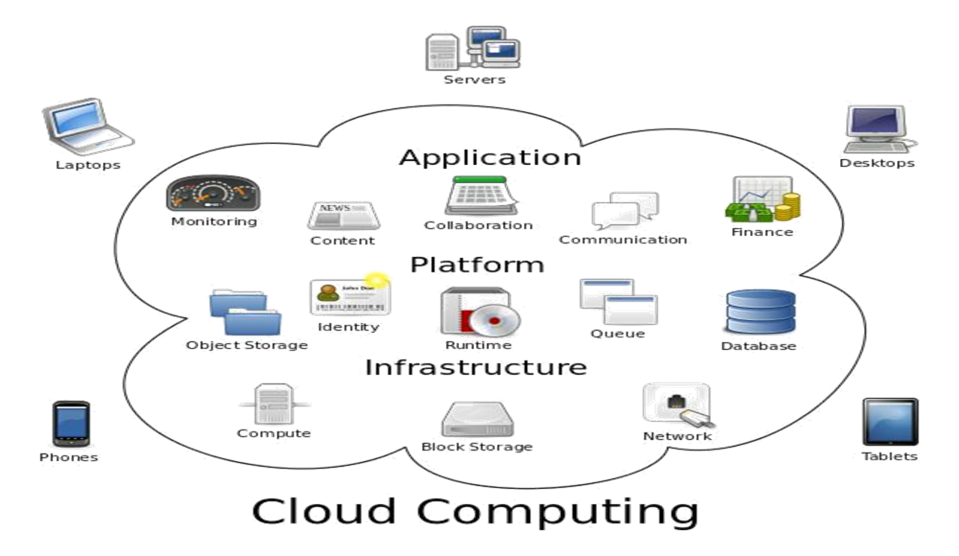
\includegraphics[width=1\linewidth]{screenshot002}
  		\caption{Le cloud compting}
  		\label{fig:screenshot002}
  	\end{figure}
  	
  	
  	\subsection{Éléments constitutifs du Cloud Computing}
  	\subsubsection{La virtualisation}
  	La virtualisation consiste à faire fonctionner un ou plusieurs systèmes d'exploitation sur un ou plusieurs ordinateurs. Cela peut sembler étrange d'installer deux systèmes d'exploitation sur une machine conçue pour en accueillir qu'un, mais comme nous le verrons par la suite, cette technique a de nombreux avantages.
  	
  	Il est courant pour des entreprises de posséder de nombreux serveurs, tels que les serveurs de mail, de nom de domaine, de stockage ...etc.
  	
  	Dans un contexte économique où il est important de rentabiliser tous les investissements, acheter plusieurs machines physiques pour héberger plusieurs serveurs n'est pas judicieux. De plus, une machine fonctionnant à 15 \% ne consomme pas plus d'énergie qu'une machine fonctionnant à 90 \%. Ainsi, regrouper ces serveurs sur une même machine peut donc s'avérer rentable si leurs pointes de charge ne coïncident pas systématiquement.
  	
  	Enfin, la virtualisation des serveurs permet une plus grande modularité dans la répartition des charges et la reconfiguration des serveurs en cas d'évolution ou de défaillance momentanée.
  	
  	\subsubsection{Datacenter}
  	Un centre de traitement de données (data centre en anglais) est un site physique sur lequel se trouvent regroupés des équipements constituants du système d'information de l'entreprise(mainframes, serveurs, baies de stockage, équipements réseaux et de télécommunications, etc.). Il peut être interne et/ou externe à l'entreprise, exploité ou non avec le soutien de prestataires. Il comprend en général un contrôle sur l'environnement (climatisation, système de prévention contre l'incendie, etc.), une alimentation d'urgence et redondante, ainsi qu'une sécurité physique élevée.
  	
  	Cette infrastructure peut être propre à une entreprise et utilisée par elle seule ou à des fins commerciales. Ainsi, des particuliers ou des entreprises peuvent venir y stocker leurs données suivant des modalités bien définies. 
  	
  \subsubsection{Plateforme collaborative}
 
 
 Une plate-forme de travail collaboratif est un espace de travail virtuel. C'est un site qui centralise tous les outils liés à la conduite d'un projet et les met à disposition des acteurs.
 
 L'objectif du travail collaboratif est de faciliter et d'optimiser la communication entre les individus dans le cadre du travail ou d'une tâche. Les plates-formes collaboratives intègrent généralement les éléments suivants :
 
 
 \begin{itemize}
\item Des outils informatiques
\item Des guides ou méthodes de travail en groupe, pour améliorer la communication, la production, la coordination.
\item 	Un service de messagerie.
\item 	Un système de partage de ressources et de fichiers.
\item 	Des outils de type forum, pages de discussions
\item 	Un trombinoscope, ou annuaire des profils des utilisateurs.
\item 	Des groupes, par projet ou par thématique.
\item 	Un calendrier. 
 
 \end{itemize}
 
 
 \subsection{Modèles de services Cloud}
 Il ya trois (03) modèles de services Cloud  \ref{fig:screenshot003} 
 \begin{figure}[h]
 	\centering
 	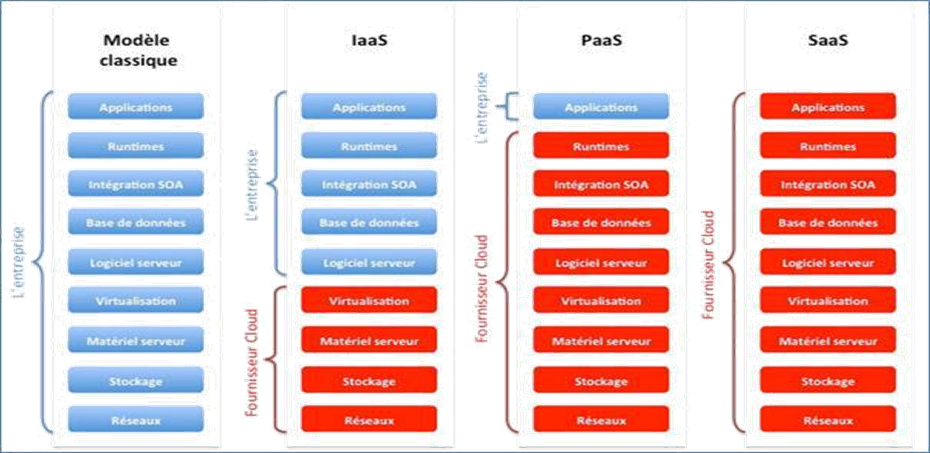
\includegraphics[width=1\linewidth]{screenshot003}
 	\caption{Modèles de services du Cloud Computing}
 	\label{fig:screenshot003}
 \end{figure}
 
 \begin{table}[h]
 
 		\centering
 		\begin{tabular}{l | l | l}
 			 & Points forts & Points faibles \\
 			\hline
 			SaaS & 12 & 13\\
 			PaaS & 22 & 14\\
 			IaaS & 23 & 12
 	
 	\end{tabular} 

 	\caption{Max and min temps recorded in the first two weeks of July}
 	\label{tab:temps}
 \end{table}
 

 Points forts	Points faibles
 SaaS	•	Pas d’installation
 •	Plus de licence	•	Logiciel limité
 •	Sécurité
 •	Dépendance de prestataire
 PaaS	•	Pas d'infrastructure Nécessaire
 •	Pas d'installation
 •	Environnement hétérogène	•	Limitation des langages
 •	Pas de personnalisation dans la configuration des machines virtuelles
 IaaS	•	Administration
 •	Personnalisation
 •	Flexibilité d'utilisation	•	Sécurité
 •	Besoin d'un administrateur système
 
 
 \section{Introduction aux Workflow:}
 